% !TEX root = ../OT4ML.tex

\chapter{Wasserstein Gradient Flows}
\index{Wasserstein!gradient}% strictindex
\index{gradient!flow}% strictindex
\index{Wasserstein!gradient flow}% strictindex
\label{sec-wasserstein-gradient-flows}

Once $\Wass_2$ is a dynamic metric, one can run gradient descent directly on the space of measures. This chapter derives the formal Wasserstein gradient, explains the JKO minimizing-movement scheme, records the role of geodesic convexity in convergence, and then applies the same calculus to mean-field neural-network training.
\index{mean-field!neural network}% strictindex
\index{minimizing movement scheme}% strictindex
\index{Wasserstein!gradient}% strictindex
\index{convexity!geodesic}% strictindex

\section{Minimizing Movements and Wasserstein Gradients}
\index{minimizing movement}% strictindex
\index{Wasserstein!gradient}% strictindex

This first section explains how a variational implicit-Euler step on measures gives rise, in the small-step limit, to a continuity equation driven by the Wasserstein gradient of the energy.
\index{Wasserstein!gradient}% strictindex
\index{continuity equation}% strictindex

We now consider a function $f(\alpha)$ and seek a minimizing evolution $(\alpha_t)_t$. The general strategy of minimizing movement over a metric space is to construct a discrete-time evolution using an implicit Euler scheme:
\index{implicit Euler scheme}% strictindex
\index{minimizing movement}% strictindex
\begin{equation}
    \alpha_{t+\tau} := \arg\min_\alpha \frac{1}{2 \tau} \Wass_2(\alpha_t, \alpha)^2 + f(\alpha). \label{eq:jko-discr}
\end{equation}

\begin{alg}[JKO minimizing movement]\label{alg:jko-minimizing-movement}
\index{JKO scheme}% strictindex
\textbf{Input:} Energy $f$, initial measure $\alpha^0$, time step $\tau>0$, number of steps $K$.

\textbf{Output:} Discrete gradient-flow trajectory $(\alpha^k)_{k=0}^K$.

\textbf{For} $k=0,\ldots,K-1$ \textbf{do}:
\begin{algblock}
\[
	\alpha^{k+1}
	\in
	\uargmin{\alpha\in\Pp_2(\RR^d)}
	\frac{1}{2\tau}\Wass_2^2(\alpha^k,\alpha)+f(\alpha).
\]
\textbf{Set} $\alpha_t^\tau=\alpha^k$ for $t\in[k\tau,(k+1)\tau)$.

\end{algblock}
\textbf{Return} $(\alpha^k)_{k=0}^K$ and $\alpha_t^\tau$.
\end{alg}

\paragraph{Euclidean gradient flows.}
\index{gradient!flow}% strictindex

If we restrict \eqref{eq:jko-discr} to finite dimensions and assume $\alpha_t = \delta_{x(t)}$ and $\alpha = \delta_x$ (single Dirac measures), this matches the implicit Euler scheme:
\index{Dirac mass}% strictindex
\index{implicit Euler scheme}% strictindex
\begin{equation*}
    x(t+\tau) := \arg\min_x \frac{1}{2 \tau} \norm{x - x(t)}^2 + h(x),
\end{equation*}
where $h(x) = f(\delta_x)$. Its solution is formally given by the implicit Euler formula:
\begin{equation*}
    x(t+\tau) = (\Id + \tau \nabla h)^{-1}(x(t)).
\end{equation*}
In contrast, the explicit Euler scheme is:
\begin{equation*}
    x(t+\tau) = (\Id - \tau \nabla h)(x(t)) = x(t) - \tau \nabla h(x(t)).
\end{equation*}

Both schemes converge as $\tau \to 0$ to:
\begin{equation}
    \dot{x}(t) = -\nabla h(x(t)). \label{eq:grad-flow-classical}
\end{equation}


\paragraph{Wasserstein gradient formula.}
\index{Wasserstein!gradient}% strictindex

The implicit Euler scheme has the advantage that it does not require $h$ or $f$ to be smooth. For $f$, this is crucial to handle evolutions over measures that may have densities, atoms or other singular parts.
\index{implicit Euler scheme}% strictindex

As $\tau \to 0$, under certain conditions on $f$, \eqref{eq:jko-discr} defines a continuous evolution $t \mapsto \alpha_t$. As discussed earlier, this evolution can be described as a Lagrangian evolution \eqref{eq:lagrangian-advection}. We use the following first-variation convention: for any $\beta\in\Pp(\RR^d)$ and the signed zero-mass perturbation $\rho=\beta-\alpha$,
\index{first variation}% strictindex
\index{signed!measure}% strictindex
\begin{equation*}
    f((1-\tau)\alpha + \tau \beta) = f(\alpha + \tau \rho) = f(\alpha) + \tau \int [\delta f(\alpha)](x) \d \rho(x) + o(\tau).
\end{equation*}
The key infinitesimal object is the vector field that represents this differential in the Wasserstein metric.

\Needspace{7\baselineskip}
\begin{defn}[Wasserstein gradient]\label{def-wasserstein-gradient}
\index{Wasserstein!gradient}% strictindex
	Assume that $f$ admits a smooth first variation $\delta f(\alpha)$. In the smooth formal calculus on $\Pp_2(\RR^d)$, the Wasserstein gradient of $f$ at $\alpha$ is the gradient vector field
	\begin{equation*}
	    \Wgrad f(\alpha) = \nabla_x \delta f(\alpha).
	\end{equation*}
\end{defn}
The associated formal gradient flow is the continuity equation
\begin{equation}
    \frac{\partial \alpha_t}{\partial t} + \diverg(-\Wgrad f(\alpha_t) \alpha_t) = 0. \label{eq:wassflow-pde}
\end{equation}
The following proposition explains why this vector field is the Riemannian gradient for the $L^2(\alpha)$ metric on velocities.
\index{signed!measure}% strictindex
%
\begin{proposition}[Formal Wasserstein gradient]\label{prop-formal-wass-gradient}
\index{Wasserstein!gradient}% strictindex
	Assume that $f$ admits a smooth first variation $\delta f(\alpha)$ and that $\alpha$ has a smooth positive density. For infinitesimal perturbations generated by a velocity field $v$ through $(\Id+\tau v)_\sharp\alpha$, the differential of $f$ is
\index{first variation}% strictindex
\index{velocity field}% strictindex
	\[
		\frac{\d}{\d\tau}_{|\tau=0}
		f\big((\Id+\tau v)_\sharp\alpha\big)
		=
		\int \dotp{\nabla \delta f(\alpha)(x)}{v(x)}\d\alpha(x).
	\]
	Hence, for the Riemannian metric $\norm{v}_{L^2(\alpha)}^2=\int \norm{v}^2\d\alpha$, the Wasserstein gradient is the vector field
\index{Wasserstein!gradient}% strictindex
	\[
		\Wgrad f(\alpha)=\nabla \delta f(\alpha).
	\]
\end{proposition}
\begin{proof}
	The push-forward expansion gives, in the sense of distributions,
\index{push-forward}% strictindex
	\[
		(\Id+\tau v)_\sharp\alpha
		=
		\alpha-\tau\diverg(\alpha v)+o(\tau).
	\]
	Using the definition of the first variation,
\index{first variation}% strictindex
	\[
		f((\Id+\tau v)_\sharp\alpha)
		=
		f(\alpha)-\tau\int \delta f(\alpha)\diverg(\alpha v)\d x+o(\tau).
	\]
	An integration by parts, with either compact support or vanishing boundary flux, gives
\index{flux}% strictindex
	\[
		-\int \delta f(\alpha)\diverg(\alpha v)\d x
		=
		\int \dotp{\nabla\delta f(\alpha)}{v}\d\alpha.
	\]
	By definition of the Riesz representative for the $L^2(\alpha)$ metric, this representative is $\nabla\delta f(\alpha)$.
\end{proof}

The Wasserstein gradient-flow viewpoint already appears in John D. Lafferty's PhD work, published as ``The Density Manifold and Configuration Space Quantization'', under the name ``density manifold''. It was then systematically developed by Otto, who exposed the formal Riemannian structure of this space~\cite{otto2001geometry}. Rigorous metric-space treatments and numerical JKO schemes can be found in~\cite{ambrosio2006gradient,JDB-JKO,2015-Peyre-siims,gallouet2017jko}.
\index{Wasserstein!gradient}% strictindex
\index{Wasserstein!gradient flow}% strictindex
\index{JKO scheme}% strictindex

%%%%
\paragraph{From the JKO step to the velocity field.}
\index{velocity field}% strictindex

A first-order expansion of the JKO step explains why~\eqref{eq:wassflow-pde} uses the vector field $\Wgrad f(\alpha)$. Write \eqref{eq:jko-discr} as a minimization over displacement fields $v$ such that $\alpha = (\Id + \tau v)_\sharp \alpha_t$:
	\[
		\min_{v} \frac{1}{2 \tau} \tau^2 \norm{v}_{L^2(\alpha_t)}^2 + f( (\Id + \tau v)_\sharp \alpha_t ).
	\]
Then we perform a first-order Taylor expansion of this formulation using
	\[
		 (\Id + \tau v)_\sharp \alpha_t =  \alpha_t - \tau \diverg( v \alpha_t ) + o(\tau)
	\]
	\[
		f( (\Id + \tau v)_\sharp \alpha_t ) = f(\alpha_t) - \tau \int \delta f(\alpha_t) \diverg( v \alpha_t ) \d x + o(\tau)
	\]
	\[
		 = f(\alpha_t) + \tau \int \langle \nabla_x \delta f(\alpha_t)(x), v(x) \rangle \d \alpha_t(x) + o(\tau)
	\]
to obtain the following first-order expansion in $\tau$ of the problem minimized in \eqref{eq:jko-discr}
	\[
		 \min_{v} f(\alpha_t) +  \tau \int \Big[ \frac{1}{2} \norm{v(x)}^2 + \langle \Wgrad f(\alpha_t)(x), v(x) \rangle \Big]\d \alpha_t(x) + o(\tau).
	\]
The pointwise minimizer is $v=-\Wgrad f(\alpha_t)$, which gives the velocity in the continuity equation.
\index{continuity equation}% strictindex
We now detail examples of such Wasserstein gradient flows.
\index{Wasserstein!gradient}% strictindex
\index{gradient!flow}% strictindex
\index{Wasserstein!gradient flow}% strictindex

\begin{figure}[ht]
\centering
\begin{tabular}{@{}cc@{}}
\small density iterates & \small quantile motion \\[-.15em]

\includegraphics[width=.43\linewidth]{figures/gradflow-jko-entropy-steps/density-steps.pdf} &

\includegraphics[width=.43\linewidth]{figures/gradflow-jko-entropy-steps/quantile-steps.pdf}
\end{tabular}
\caption{JKO minimizing movements for the entropy flow in one dimension. The left panel displays successive implicit-Euler minimizers for the heat equation, colored from red to blue. The right panel tracks inverse CDF values $Q_t(s)=F_t^{-1}(s)$ for selected probability levels $s$, giving a Lagrangian view of the proximal movement in Wasserstein space.}
\index{minimizing movement}% strictindex
\index{Wasserstein!space}% strictindex
\index{heat equation}% strictindex
\label{fig:gradflow-jko-entropy-steps}
\end{figure}

%%%
\paragraph{Discrete evolutions.}
\index{measure!evolution}% strictindex

If $f(\alpha)$ can be evaluated on discrete distributions and $\Wgrad$ is continuous in this case, the flow \eqref{eq:wassflow-pde} maintains the number of Dirac masses, $\alpha_t = \frac{1}{n} \sum_i \delta_{x_i(t)}$. The particles $X(t) := (x_i(t))_i$ evolve according to a system of coupled ODEs:
\index{Dirac mass}% strictindex
\begin{equation}
    \dot{x}_i(t) = -n\nabla_{x_i} F(X(t)), \label{eq:wassflows-particles}
\end{equation}
where $F(X) := f\left(\frac{1}{n} \sum_i \delta_{x_i}\right)$ and the factor $n$ comes from the empirical Wasserstein metric $\frac1n\sum_i \norm{\dot x_i}^2$.

\begin{alg}[Empirical Wasserstein particle descent]\label{alg:empirical-wasserstein-particle-flow}
\index{particle!Wasserstein descent}% strictindex
\textbf{Input:} Particles $X^0=(x_1^0,\ldots,x_n^0)$, functional $f$, step size $h$.

\textbf{Output:} Particle trajectory $(X^k)_k$ and empirical measures.

\textbf{Define}
\[
	F(X)=f\!\left(\frac1n\sum_{i=1}^n\delta_{x_i}\right).
\]
\textbf{For} $k=0,1,\ldots$ \textbf{do}:
\begin{algblock}

\textbf{For} $i=1,\ldots,n$ \textbf{do}
\begin{algblock}
\[
	g_i^k=n\nabla_{x_i}F(X^k),
	\qquad
	x_i^{k+1}=x_i^k-h\,g_i^k.
\]
\end{algblock}
\textbf{If} stopping criterion is met \textbf{then}:
\begin{algblock}

\textbf{Return} $\frac1n\sum_i\delta_{x_i^k}$.

\end{algblock}
\end{algblock}
\end{alg}

%%%
\paragraph{Linear Functionals.}
\index{linear!functional}% strictindex

The first benchmark is a functional whose first variation does not depend on the current measure.

\begin{example}[Linear potentials generate independent particles]
Take a linear functional
   \begin{equation}\label{eq:linear-func}
       f(\alpha) = \int h(x) \d \alpha(x).
   \end{equation}
   Then $\delta f(\alpha) = h$ is independent of $\alpha$, and the flow \eqref{eq:wassflow-pde} becomes
   \begin{equation*}
       \frac{\partial \alpha_t}{\partial t} + \diverg(-\nabla h \alpha_t) = 0.
   \end{equation*}
   This implies particles move independently according to the usual gradient flow \eqref{eq:grad-flow-classical}.
\index{gradient!flow}% strictindex
\end{example}

%%%
\paragraph{Shannon Neg-Entropy.}
\index{Shannon!negative entropy}% strictindex


Entropy gives the opposite benchmark: the flow is no longer a deterministic push-forward of particles, but a diffusion of density.

\begin{example}[Entropy generates heat and porous-medium flows]
The canonical density-dependent functional is the Shannon neg-entropy
   \begin{equation}
       f(\alpha) = \int \log\left(\frac{\d \alpha}{\d x}(x)\right) \d \alpha(x). \label{eq:entropy-func}
   \end{equation}
   Here, $\delta f(\alpha) = \log(\d\alpha/\d x)$ up to an additive constant, so $\Wgrad f(\alpha) = \nabla \alpha/\alpha$ (often called the score). The flow \eqref{eq:wassflow-pde} becomes the heat equation
\index{score function}% strictindex
\index{heat equation}% strictindex
   \begin{equation*}
       \partial_t \alpha_t = \Delta \alpha_t.
   \end{equation*}
   Other entropy functionals lead to nonlinear diffusion equations; finite-volume and particle discretizations are discussed in~\cite{CarrilloFiniteVolume,GianazzaARMA,Maas2011,ErbarHeatManifold}.
%
For a generalized entropy
   \begin{equation}\label{eq:gen-entropies}
       f(\alpha) = \int g\left(\frac{\d \alpha}{\d x}\right) \d x,
   \end{equation}
	   with a scalar convex function $g$, one obtains nonlinear diffusions in the smooth-density regime:
\index{convex!function}% strictindex
   \begin{equation*}
       \frac{\partial \alpha_t}{\partial t} = \Delta(P(\alpha_t)),
   \end{equation*}
   where the pressure $P$ satisfies $P'(s)=s g''(s)$. For example, $g(s) = s \log(s)$ gives $P(s)=s$ and recovers \eqref{eq:entropy-func}, while $g(s) = s^m/(m-1)$, $m > 1$, gives $P(s)=s^m$ up to an additive constant and yields the porous-medium equation.
\index{porous medium equation}% strictindex
\end{example}
	%
The preceding examples are also governed by a precise geodesic-convexity criterion.
	A celebrated theorem by McCann~\cite{mccann1997convexity} states that an internal energy of the form~\eqref{eq:gen-entropies}, for $g : \RR^+ \to \RR\cup\{+\infty\}$ with $g(0)=0$, is geodesically convex on $\Pp(\RR^d)$ when $g$ is convex and the map $r \mapsto r^d g(r^{-d})$ is convex and nonincreasing on $(0,+\infty)$.
	%
	Examples of such functions are $g(s)=s^q$ for $q>1$ and Shannon entropy $g(s)=s \log(s)$. %
\index{Shannon!entropy}% strictindex
	By contrast, $g(s)=-\log(s)$, associated with the reverse KL divergence, does not satisfy this displacement-convexity criterion.
\index{reverse KL divergence}% strictindex
\index{displacement!convexity}% strictindex

\begin{figure}[ht]
\centering
\begin{tabular}{@{}ccc@{}}
\small heat equation & \small porous medium $m=2$ & \small porous medium $m=6$ \\[-.15em]
\index{heat equation}% strictindex
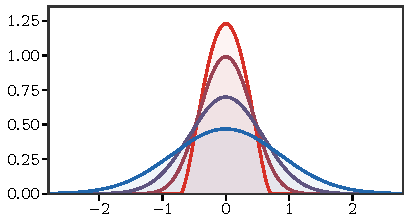
\includegraphics[width=.30\linewidth]{figures/gradflow-heat-versus-porous-medium/heat.pdf} &
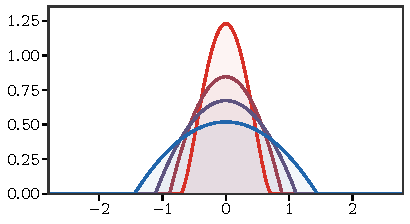
\includegraphics[width=.30\linewidth]{figures/gradflow-heat-versus-porous-medium/porous-medium.pdf} &
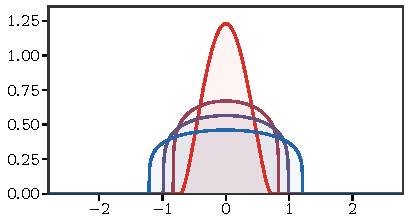
\includegraphics[width=.30\linewidth]{figures/gradflow-heat-versus-porous-medium/porous-medium-m6.pdf}
\end{tabular}
\caption{Entropy-driven Wasserstein gradient flows from the same compact initial density. The heat flow is generated by Shannon entropy $g(\rho)=\rho\log\rho$ and instantly develops Gaussian tails. The porous-medium flows use the power entropy $g(\rho)=\rho^m/(m-1)$, hence $\partial_t\rho=\Delta(\rho^m)$: the middle panel has $m=2$, while the right panel has the stronger nonlinearity $m=6$, i.e. $\partial_t\rho=\Delta(\rho^6)$. Larger powers diffuse mainly where the density is high, producing a flatter core and a sharper compact free boundary.}
\index{Wasserstein!gradient flow}% strictindex
\index{Shannon!entropy}% strictindex
\label{fig:gradflow-heat-versus-porous-medium}
\end{figure}

%%%
\paragraph{Interaction Energies.}
\index{energy!interaction}% strictindex

In a similar spirit, to obtain nonlinear evolutions without requiring the measure to have density, one can consider
   \begin{equation}
       f(\alpha) := \iint k(x, y) \d \alpha(x) \d \alpha(y). \label{eq:quadratic-func}
   \end{equation}
   For a symmetric kernel $k$:
   \begin{equation*}
       \delta f(\alpha)(x) = 2 \int k(x, y) \d \alpha(y), \quad \Wgrad f(\alpha)(x) = 2 \int \nabla_x k(x, y) \d \alpha(y).
   \end{equation*}
   For $\alpha_0 = \frac{1}{n} \sum_i \delta_{x_i}$, the flow \eqref{eq:wassflow-pde} implies particles $(x_i(t))_i$ obey:
   \begin{equation*}
       \dot{x}_i(t) = -\frac{2}{n} \sum_j \nabla k(x_i(t), x_j(t)).
   \end{equation*}
	   If $k$ is positive definite, or more generally conditionally positive definite on signed measures of zero total mass as for the energy-distance kernel $k(x,y)=-\norm{x-y}$, and one minimizes the squared kernel discrepancy to a teacher distribution $\beta$, then
\index{teacher distribution}% strictindex
\index{energy!distance}% strictindex
\index{signed!measure}% strictindex
   \[
       \norm{\alpha-\beta}_k^2
       =
       \iint k\d\alpha\d\alpha
       -2\int\!\left(\int k(x,y)\d\beta(y)\right)\d\alpha(x)
       +\mathrm{constant}.
       \]
	       Thus MMD-type training energies are exactly an interaction energy plus a linear potential; the teacher distribution appears through the potential $x\mapsto-2\int k(x,y)\d\beta(y)$. The corresponding empirical Wasserstein gradient flow is
\index{teacher distribution}% strictindex
\index{Wasserstein!gradient}% strictindex
\index{gradient!flow}% strictindex
\index{maximum mean discrepancy}% strictindex
\index{Wasserstein!gradient flow}% strictindex
\index{energy!interaction}% strictindex
       \[
		\dot x_i(t)
		=
		-\frac{2}{n}\sum_j\nabla_x k(x_i(t),x_j(t))
		+
		2\int\nabla_x k(x_i(t),y)\d\beta(y).
       \]

The corresponding simulation loop is Algorithm~\ref{alg:mmd-particle-flow}.

\begin{alg}[MMD particle flow against a teacher law]\label{alg:mmd-particle-flow}
\index{maximum mean discrepancy}% strictindex
\textbf{Input:} Initial particles $(x_i^0)_{i=1}^n$, teacher law $\beta$, kernel $k$, step size $h$.

\textbf{Output:} Particle trajectory targeting $\beta$.

\textbf{For} $k=0,1,\ldots$ \textbf{do}:
\begin{algblock}

\textbf{For} $i=1,\ldots,n$ \textbf{do}
\begin{algblock}
\[
	v_i^k
	=
	-\frac{2}{n}\sum_{j=1}^n\nabla_x k(x_i^k,x_j^k)
	+
	2\int\nabla_x k(x_i^k,y)\d\beta(y).
\]
\textbf{If} the teacher integral is unavailable \textbf{then}:
\begin{algblock}

\textbf{Set} teacher integral by quadrature/minibatch estimation.

\end{algblock}
\textbf{Update}
\[
	x_i^{k+1}=x_i^k+h\,v_i^k.
\]
\end{algblock}
\end{algblock}
\textbf{Return} $(x_i^k)_{i,k}$.
\end{alg}

	       The first term is a kernelized self-interaction, while the second is the attraction induced by the continuous teacher kernel mean. At the continuum level, characteristic positive-definite kernels, and the Euclidean energy-distance kernel on probability measures, have $\beta$ as the unique minimizer of $\norm{\alpha-\beta}_k^2$. For a finite number of particles, however, the flow can only form a kernelized quadrature of $\beta$, and small particle systems may cover the target modes poorly. Figure~\ref{fig:gradflow-mmd-particle-count} illustrates this finite-particle effect.
\index{kernelized self-interaction}% strictindex
\index{teacher kernel mean}% strictindex
\index{characteristic kernel}% strictindex
\index{kernel quadrature}% strictindex
\index{probability measure}% strictindex
\index{kernel!positive definite}% strictindex
\index{energy!distance}% strictindex

\begin{figure}[ht]
\centering
\begin{tabular}{@{}ccc@{}}
\small $n=10$ particles & \small $n=50$ particles & \small $n=300$ particles \\[-.15em]
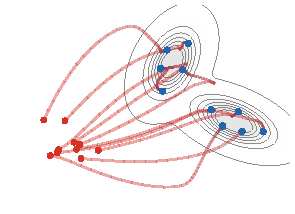
\includegraphics[width=.30\linewidth]{figures/gradflow-mmd-particle-count/n-010.pdf} &
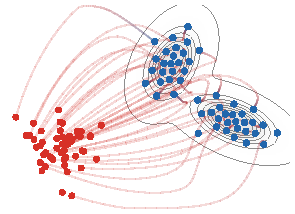
\includegraphics[width=.30\linewidth]{figures/gradflow-mmd-particle-count/n-050.pdf} &
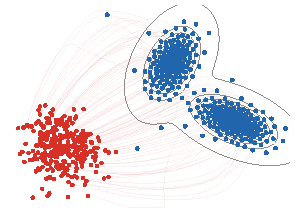
\includegraphics[width=.30\linewidth]{figures/gradflow-mmd-particle-count/n-300.pdf}
\end{tabular}
\caption{Particle count in the deterministic Wasserstein gradient flow of the squared MMD-type discrepancy to a smooth two-Gaussian teacher distribution, using here the energy-distance kernel $k(x,y)=-\norm{x-y}$. The teacher itself is shown only through true density contours, while red dots are a compact shifted Gaussian initialization placed away from the target, red-to-blue curves show a thinned subset of particle trajectories, and blue dots show the stabilized long-time particles. With too few particles, the empirical measure forms a sparse kernelized quadrature and may under-cover the target modes; increasing $n$ makes the particle cloud approximate the continuous target geometry more faithfully.}
\index{teacher distribution}% strictindex
\index{kernel quadrature}% strictindex
\index{Wasserstein!gradient flow}% strictindex
\index{empirical!measure}% strictindex
\index{energy!distance}% strictindex
\label{fig:gradflow-mmd-particle-count}
\end{figure}

\begin{figure}[ht]
\centering
\begin{tabular}{@{}ccc@{}}
\small repulsive kernel & \small attractive kernel & \small attraction--repulsion \\[-.15em]

\includegraphics[width=.30\linewidth]{figures/gradflow-interaction-particles/repulsive.pdf} &

\includegraphics[width=.30\linewidth]{figures/gradflow-interaction-particles/attractive.pdf} &
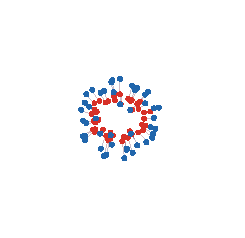
\includegraphics[width=.30\linewidth]{figures/gradflow-interaction-particles/attraction-repulsion.pdf}
\end{tabular}
\caption{Interaction-energy particle flows for three choices of $k$. A positive Gaussian kernel $k(x,y)=\exp(-\norm{x-y}^2/(2\sigma^2))$ produces short-range repulsion under Wasserstein descent; changing its sign produces attraction and collapse; adding a quadratic long-range attraction to the repulsive kernel yields a balanced attraction--repulsion dynamics. The curves use arclength-based red-to-blue coloring along a longer integration of the coupled particle ODE~\eqref{eq:wassflows-particles}.}
\index{particle ODE}% strictindex
\index{energy!interaction}% strictindex
\label{fig:gradflow-interaction-particles}
\end{figure}

\begin{figure}[ht]
\centering
\begin{tabular}{@{}cccc@{}}
\small OT rays & \small MMD force & \small Sinkhorn force & \small drifting field \\[-.15em]

\includegraphics[width=.225\linewidth]{figures/gradflow-particle-objective-geometries/ot-rays.pdf} &

\includegraphics[width=.225\linewidth]{figures/gradflow-particle-objective-geometries/mmd-force.pdf} &

\includegraphics[width=.225\linewidth]{figures/gradflow-particle-objective-geometries/sinkhorn-divergence.pdf} &
\index{Sinkhorn!divergence}% strictindex
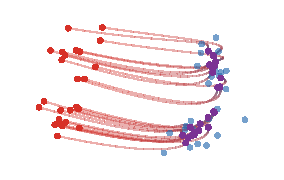
\includegraphics[width=.225\linewidth]{figures/gradflow-particle-objective-geometries/drifting-field.pdf}
\end{tabular}
\caption{Particle trajectories induced by different discrepancy geometries. The red particles and blue target cloud are the same in all panels. Straight OT displacement produces rays from an optimal matching; an MMD-type witness field gives smoother nonlocal forces; the Sinkhorn-divergence force is an entropic, debiased transport attraction; and the normalized drifting field combines attraction to data with self-repulsion. The figure is qualitative: it compares geometric behavior, not solver performance.}
\label{fig:gradflow-particle-objective-geometries}
\end{figure}

\paragraph{Stochastic particles and McKean--Vlasov limits.}
\index{stochastic!particle}% strictindex
\index{McKean-Vlasov limit}% strictindex
More generally, deterministic particle flows have stochastic counterparts, where Brownian noise at the particle level becomes an entropy term at the level of measures. If the drift does not depend on the empirical measure, each particle evolves independently according to
\index{empirical!measure}% strictindex
\[
	\d X_t=b(X_t)\d t+\sqrt{2}\sigma\d B_t,
\]
and the one-particle law $\alpha_t=\rho_t\d x$ directly satisfies the linear Fokker--Planck equation
\index{Fokker-Planck equation}% strictindex
\[
	\partial_t\rho_t=-\diverg(b\rho_t)+\sigma^2\Delta\rho_t.
\]

\begin{example}[Langevin drift as a free-energy flow]
	If $b=-\nabla V$, this linear Fokker--Planck equation is the $\Wass_2$ gradient flow of the free energy
	\[
		\rho\mapsto \int V\rho\,\d x+\sigma^2\int\rho\log\rho\,\d x.
	\]
\end{example}

The mean-field case is different: the drift is recomputed from the current empirical distribution of all particles,
\index{empirical!distribution}% strictindex
\index{gradient!flow}% strictindex
\[
	\d X_i^n(t)=b(X_i^n(t),\mu_t^n)\d t+\sqrt{2}\sigma\d B_i(t),
	\qquad
	\mu_t^n=\frac1n\sum_{i=1}^n\delta_{X_i^n(t)} .
\]
For finite $n$, the empirical law $\mu_t^n$ is itself random. Under suitable Lipschitz, growth and chaotic-initialization assumptions, propagation of chaos states that finitely many particles become asymptotically independent as $n\to\infty$, all with the same deterministic law $\rho_t\d x$; equivalently, the empirical measure $\mu_t^n$ converges in probability to this law. The limiting density solves the nonlinear Fokker--Planck, or McKean--Vlasov, equation
\index{Fokker-Planck equation}% strictindex
\index{McKean-Vlasov limit}% strictindex
\index{propagation of chaos}% strictindex
\index{empirical!law}% strictindex
\[
	\partial_t \rho_t
	=
	-\diverg\big(b(x,\rho_t)\rho_t\big)
	+
	\sigma^2\Delta\rho_t .
\]
When the interaction drift has variational form
\[
	b(x,\rho)=-\nabla \frac{\delta \mathcal E}{\delta \rho}(x),
\]
	this PDE is the Wasserstein gradient flow of the entropy-regularized energy
\index{Wasserstein!gradient}% strictindex
\index{gradient!flow}% strictindex
\index{Wasserstein!gradient flow}% strictindex
	\[
		\mathcal E(\rho)+\sigma^2\int \rho\log\rho\,\d x .
	\]

\begin{figure}[ht]
\centering
\begin{tabular}{@{}c@{}}
\small independent Langevin particles \\[-.15em]
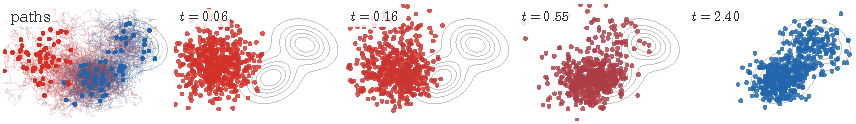
\includegraphics[width=.86\linewidth]{figures/gradflow-fokker-planck-three-representations/langevin-particles.pdf} \\[.25em]
\small deterministic KDE-score particles \\[-.15em]
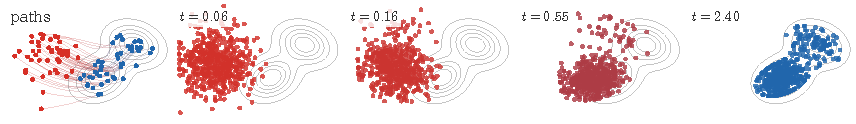
\includegraphics[width=.86\linewidth]{figures/gradflow-fokker-planck-three-representations/kde-particles.pdf} \\[.25em]
\small grid Fokker--Planck density \\[-.15em]
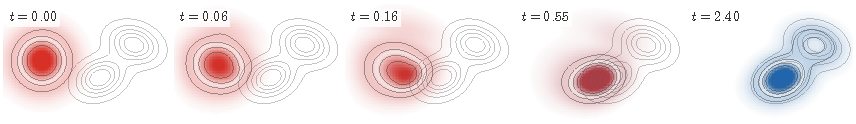
\includegraphics[width=.86\linewidth]{figures/gradflow-fokker-planck-three-representations/grid-pde.pdf}
\end{tabular}
\caption{Three numerical representations of the same entropy-regularized Wasserstein gradient flow of $\KL(\rho|\beta)$, where $\beta$ is a two-Gaussian target shifted to the right of an initially isotropic Gaussian density. The first row simulates independent Langevin particles and displays a thinned set of trajectories in the left panel. The second row evolves many deterministic particles with velocity $\tau(\nabla\log\beta-\nabla\log\rho_t)$, estimating $\nabla\log\rho_t$ by a sharper kernel-density score; only representative trajectories and particle subsets are displayed. The third row solves the corresponding Fokker--Planck equation on a grid, starting from the initial density in the left panel. The remaining columns use front-loaded times, so that the onset of the flow and the later deformation toward a bimodal law are both visible.}
\index{Wasserstein!gradient flow}% strictindex
\index{Fokker-Planck equation}% strictindex
\label{fig:gradflow-fokker-planck-three-representations}
\end{figure}

\section{Geodesic Convexity and Convergence}
\index{convexity!geodesic}% strictindex
\label{sec-geodesic-convexity}

Geodesic convexity is the convexity notion adapted to Wasserstein geometry. It is the condition that turns the formal gradient-flow calculus into a convergence theory.
\index{convexity!geodesic}% strictindex
\index{gradient!flow}% strictindex

\paragraph{Geodesics and convexity.}

A constant-speed $\Wass_2$ geodesic between $\alpha_0$ and $\alpha_1$ is obtained, as in Definition~\ref{def-w2-geodesic-induced-by-plan}, from any optimal coupling $\pi^\star\in\Couplings(\alpha_0,\alpha_1)$ by the McCann interpolation
\index{optimal coupling}% strictindex
\index{constant-speed geodesic}% strictindex
\index{McCann interpolation}% strictindex
\[
	\alpha_t=((1-t)P_0+tP_1)_\sharp\pi^\star,
	\qquad t\in[0,1],
\]
where $P_0(x,y)=x$ and $P_1(x,y)=y$. If the optimal plan is induced by a Brenier map $T$, this reduces to $((1-t)\Id+tT)_\sharp\alpha_0$. The coupling formula is important because geodesics exist even when no Monge map exists, for instance when a Dirac mass must split.
\index{Monge!problem}% strictindex
\index{optimal plan}% strictindex
\index{Brenier!map}% strictindex
\index{Dirac mass}% strictindex

\begin{defn}[Geodesic convexity]\label{def-geodesic-convexity}
\index{convexity!geodesic}% strictindex
	A functional $f$ on $\Pp_2(\RR^d)$ is geodesically convex if for every $\Wass_2$ geodesic $(\alpha_t)_t$,
	\[
		f(\alpha_t)\leq (1-t)f(\alpha_0)+t f(\alpha_1).
	\]
	It is $\lambda$-geodesically convex if the right-hand side is improved by $-\frac{\lambda}{2}t(1-t)\Wass_2^2(\alpha_0,\alpha_1)$.
\end{defn}

\begin{prop}[Basic geodesically convex energies]\label{prop-basic-geodesic-convexity}
\index{convexity!geodesic}% strictindex
	The following formal statements hold on $\Pp_2(\RR^d)$.
	\begin{enumerate}
		\item If $h$ is convex, then $\alpha\mapsto\int h\d\alpha$ is geodesically convex; if $h$ is $\lambda$-strongly convex, it is $\lambda$-geodesically convex.
		\item If $W(x-y)$ is convex as a function of the displacement, then $\alpha\mapsto\frac12\iint W(x-y)\d\alpha(x)\d\alpha(y)$ is geodesically convex.
		\item Shannon entropy $\alpha\mapsto\int\rho\log\rho\,\d x$ is geodesically convex.
\index{Shannon!entropy}% strictindex
		\item The relative entropy $\KL(\alpha|\gamma)$ with $\d\gamma=e^{-V}\d x/Z$ is $\lambda$-geodesically convex when $V$ is $\lambda$-strongly convex.
\index{entropy!relative}% strictindex
	\end{enumerate}
\end{prop}
\begin{proof}
	Along a Monge geodesic $X_t=(1-t)X_0+tX_1$, convexity of $h$ gives $h(X_t)\leq(1-t)h(X_0)+t h(X_1)$, and strong convexity gives the additional quadratic term; integrating proves the first claim. The interaction claim follows similarly by applying convexity of $W$ to pairwise differences $X_t-X_t'=(1-t)(X_0-X_0')+t(X_1-X_1')$ and integrating over two independent copies. The entropy claim is McCann's displacement convexity theorem; at the density level it follows from the concavity of the Jacobian determinant under the interpolation of optimal maps. Finally, $\KL(\alpha|\gamma)=\int\rho\log\rho\,\d x+\int V\d\alpha+\mathrm{constant}$, so it is the sum of displacement-convex entropy and a $\lambda$-geodesically convex linear potential.
\index{displacement!convexity}% strictindex
\index{Jacobian determinant}% strictindex
\index{convexity!geodesic}% strictindex
\index{Monge!geodesic}% strictindex
\end{proof}

\paragraph{Convergence of the flow.}

In general, analyzing \eqref{eq:wassflow-pde} is delicate. The cleanest case is when $f$ is geodesically convex in the sense above. This condition is the Wasserstein analogue of convexity in Euclidean gradient descent.

\begin{prop}[Energy decay for convex Wasserstein flows]\label{prop-convex-wass-flow-rate}
\index{energy!decay}% strictindex
\index{Wasserstein!flow}% strictindex
	Assume formally that $f$ is geodesically convex, admits a smooth first variation, and has a minimizer $\alpha^\star$. Let $(\alpha_t)_t$ be a smooth solution of the Wasserstein gradient flow
\index{first variation}% strictindex
\index{Wasserstein!gradient}% strictindex
\index{gradient!flow}% strictindex
\index{Wasserstein!gradient flow}% strictindex
	\[
		\partial_t\alpha_t+\diverg(\alpha_t v_t)=0,
		\qquad
		v_t=-\Wgrad f(\alpha_t).
	\]
	Then
	\[
		\frac{\d}{\d t} f(\alpha_t)
		=
		-\int \norm{\Wgrad f(\alpha_t)(x)}^2\,\d\alpha_t(x)
		\leq 0.
	\]
	If $T_t$ is the optimal map from $\alpha_t$ to $\alpha^\star$, then
	\[
		f(\alpha_t)-f(\alpha^\star)
		\leq
		-\frac{\d}{\d t}\frac12 \Wass_2^2(\alpha_t,\alpha^\star),
	\]
	and consequently
	\[
		f(\alpha_t)-f(\alpha^\star)
		\leq
		\frac{\Wass_2^2(\alpha_0,\alpha^\star)}{2t}.
	\]
	If $f$ is $\lambda$-geodesically convex with $\lambda>0$, then
	\[
		f(\alpha_t)-f(\alpha^\star)
		\leq
		e^{-2\lambda t}\bigl(f(\alpha_0)-f(\alpha^\star)\bigr).
	\]
\end{prop}

\begin{proof}
	The chain rule and Proposition~\ref{prop-formal-wass-gradient} give
	\[
		\frac{\d}{\d t}f(\alpha_t)
		=
		\int \dotp{\Wgrad f(\alpha_t)(x)}{v_t(x)}\,\d\alpha_t(x)
		=
		-\int \norm{\Wgrad f(\alpha_t)(x)}^2\,\d\alpha_t(x).
	\]
	Geodesic convexity along the geodesic
\index{convexity!geodesic}% strictindex
	$((1-s)\Id+sT_t)_\sharp\alpha_t$ gives
	\[
		f(\alpha^\star)-f(\alpha_t)
		\geq
		\int \dotp{\Wgrad f(\alpha_t)(x)}{T_t(x)-x}\,\d\alpha_t(x).
	\]
	Since $v_t=-\Wgrad f(\alpha_t)$, this reads
	\[
		f(\alpha_t)-f(\alpha^\star)
		\leq
		\int \dotp{v_t(x)}{T_t(x)-x}\,\d\alpha_t(x).
	\]
	The standard first-variation formula for the squared Wasserstein distance gives
\index{Wasserstein!distance}% strictindex
	\[
		\frac{\d}{\d t}\frac12\Wass_2^2(\alpha_t,\alpha^\star)
		=
		\int \dotp{x-T_t(x)}{v_t(x)}\,\d\alpha_t(x),
	\]
	which proves the differential inequality. Integrating it from $0$ to $t$ and using the monotonicity of $s\mapsto f(\alpha_s)$ gives
	\[
		t\bigl(f(\alpha_t)-f(\alpha^\star)\bigr)
		\leq
		\int_0^t \bigl(f(\alpha_s)-f(\alpha^\star)\bigr)\,\d s
		\leq
		\frac12\Wass_2^2(\alpha_0,\alpha^\star).
	\]
	If $f$ is $\lambda$-geodesically convex, the Wasserstein analogue of strong convexity gives the slope inequality
	\[
		\int\norm{\Wgrad f(\alpha_t)}^2\d\alpha_t
		\geq
		2\lambda\bigl(f(\alpha_t)-f(\alpha^\star)\bigr).
	\]
	Combining it with the energy dissipation identity yields
\index{energy!dissipation}% strictindex
	\[
		\frac{\d}{\d t}\bigl(f(\alpha_t)-f(\alpha^\star)\bigr)
		\leq
		-2\lambda\bigl(f(\alpha_t)-f(\alpha^\star)\bigr),
	\]
	and Gronwall's lemma gives the exponential rate.
\end{proof}

\begin{prop}[Convex examples covered by the theory]\label{prop-convex-flow-examples}
	The hypotheses of Proposition~\ref{prop-convex-wass-flow-rate} are satisfied in the following standard cases, at least at the formal smooth level used in this section.
	\begin{enumerate}
		\item For the linear energy $f(\alpha)=\int h\d\alpha$, geodesic convexity holds when $h$ is convex. If $h$ is $\lambda$-strongly convex, then $f$ is $\lambda$-geodesically convex and the flow enjoys the exponential rate of Proposition~\ref{prop-convex-wass-flow-rate}.
\index{convexity!geodesic}% strictindex
		\item For the interaction energy $f(\alpha)=\frac12\iint W(x-y)\d\alpha(x)\d\alpha(y)$, geodesic convexity holds when $W$ is convex and even. This covers repulsive or attractive pairwise models whose displacement cost has no non-convex wells.
\index{energy!interaction}% strictindex
		\item The Shannon entropy $f(\alpha)=\int\rho\log\rho\,\d x$ and, more generally, McCann displacement-convex internal energies generate diffusion-type Wasserstein gradient flows.
\index{Wasserstein!gradient}% strictindex
\index{gradient!flow}% strictindex
\index{Wasserstein!gradient flow}% strictindex
\index{Shannon!entropy}% strictindex
		\item If $\gamma=Z^{-1}e^{-V}\d x$ and $V$ is $\lambda$-strongly convex, then the relative entropy $\KL(\alpha|\gamma)$ is $\lambda$-geodesically convex. Its flow is the Fokker--Planck equation with invariant law $\gamma$.
\index{Fokker-Planck equation}% strictindex
\index{entropy!relative}% strictindex
	\end{enumerate}
\end{prop}
\begin{proof}
	Let $(\alpha_t)_t$ be the McCann interpolation between $\alpha_0$ and $\alpha_1$, written with an optimal coupling as $X_t=(1-t)X_0+tX_1$. For a linear energy, Jensen's inequality gives
\index{Jensen inequality}% strictindex
\index{optimal coupling}% strictindex
\index{McCann interpolation}% strictindex
	\[
		h(X_t)\leq(1-t)h(X_0)+t h(X_1),
	\]
	and the strong convexity version gives the additional term $-\frac{\lambda}{2}t(1-t)\norm{X_0-X_1}^2$. Integrating over the optimal coupling proves geodesic convexity and $\lambda$-geodesic convexity.
\index{convexity!geodesic}% strictindex

	For interaction energies, use two independent copies of the optimal coupling. The pairwise displacement evolves as
\index{optimal coupling}% strictindex
\index{energy!interaction}% strictindex
	\[
		X_t-X_t'=(1-t)(X_0-X_0')+t(X_1-X_1').
	\]
	Convexity of $W$ gives the convexity inequality after integration over the product coupling. Evenness of $W$ ensures that the interaction is symmetric in the two particles and matches the usual factor $1/2$ in~\eqref{eq:quadratic-func}.
\index{product!coupling}% strictindex

	The entropy claim is McCann's displacement-convexity theorem. For smooth positive densities and Brenier maps, it follows from the change-of-variables formula and the concavity of the determinant along positive matrices; the general statement is obtained by approximation. Finally,
\index{change-of-variables}% strictindex
\index{change-of-variables formula}% strictindex
\index{displacement!convexity}% strictindex
\index{Brenier!map}% strictindex
	\[
		\KL(\alpha|\gamma)=\int\rho\log\rho\,\d x+\int V\d\alpha+\log Z,
	\]
	so it is the sum of the displacement-convex entropy and the $\lambda$-geodesically convex linear potential generated by $V$. Proposition~\ref{prop-convex-wass-flow-rate} then applies to all four cases.
\end{proof}

\paragraph{Convexity and curvature.}

The same language is not restricted to subsets of $\RR^d$. If $(\X,\dist,\mathfrak m)$ is a geodesic metric-measure space, $\Wass_2$ geodesics can be defined by transporting each pair of endpoints along metric geodesics, or more intrinsically by dynamical optimal plans on path space, as discussed in Section~\ref{sec-kantorovich-plan-interpolation}. Given a reference measure $\mathfrak m$, the entropy relative to $\mathfrak m$ is
\index{metric-measure space}% strictindex
\index{geodesic!space}% strictindex
\index{entropy!relative}% strictindex
\index{dynamical optimal plan}% strictindex
\[
	\mathrm{Ent}_{\mathfrak m}(\alpha)
	\eqdef
	\begin{cases}
		\displaystyle \int_\X \rho\log\rho\,\d\mathfrak m,
		& \text{if } \alpha=\rho\,\mathfrak m,\\
		+\infty,
		& \text{otherwise.}
	\end{cases}
\]
On a smooth Riemannian manifold $(M,g)$, the Ricci curvature tensor $\mathrm{Ric}_g$ is the trace of the Riemann curvature tensor; the lower bound $\mathrm{Ric}_g\geq\lambda g$ means that $\mathrm{Ric}_g(v,v)\geq\lambda |v|_g^2$ for every tangent vector $v$. The fundamental link between curvature and optimal transport is that this tensor lower bound is exactly encoded by geodesic convexity of entropy.
\index{Ricci curvature}% strictindex
\index{Riemannian manifold}% strictindex
\index{convexity!geodesic}% strictindex

\begin{thm}[Ricci curvature and entropy convexity]\label{thm-ricci-entropy-convexity}
\index{Ricci curvature}% strictindex
\index{entropy!relative}% strictindex
\index{convexity!geodesic}% strictindex
	Let $(M,g)$ be a smooth compact connected Riemannian manifold without boundary, and let $\mathfrak m=\mathrm{vol}_g$. For $\lambda\in\RR$, the lower Ricci bound $\mathrm{Ric}_g\geq\lambda g$ holds if and only if $\mathrm{Ent}_{\mathfrak m}$ is $\lambda$-geodesically convex on $(\Pp_2(M),\Wass_2)$.
\end{thm}

This equivalence was developed in the smooth Riemannian setting by Cordero-Erausquin, McCann and Schmuckenschl{\"a}ger and by von Renesse and Sturm~\cite{cordero2001riemannian,vonrenesse2005transport}; it is a central theme of the optimal-transport approach to curvature in Villani's monograph~\cite{Villani09}. Lott--Villani and Sturm then used the same entropy-convexity principle to define synthetic lower Ricci curvature bounds on metric-measure spaces~\cite{lott2009ricci,sturm2006geometry1,sturm2006geometry2}. Outside this convex, curvature-controlled regime, such as in the mean-field neural-network example below, the flow may still be informative but its convergence analysis requires problem-specific arguments.
\index{metric-measure space}% strictindex
\index{synthetic Ricci curvature}% strictindex
\index{mean-field!neural network}% strictindex


\section{Training Two-Layer MLPs as Wasserstein Flows}

Mean-field limits recast the training of wide neural networks as transport of a distribution of neurons. This section shows how the particle ODE of gradient descent becomes a Wasserstein flow in parameter space.
\index{particle ODE}% strictindex
\index{neuron}% strictindex
\index{mean-field!limit}% strictindex

We use $z\in\RR^d$ for the input data and $y\in\RR^{d'}$ for the label. A neuron is a particle
\[
	x=(u,v)\in\RR^d\times\RR^{d'},
\]
where $u$ is the inner weight and $v$ is the outer vector weight. For a scalar nonlinearity $\sigma$, define the vector-valued feature
\[
	\psi(x,z)=v\,\sigma(\dotp{u}{z})\in\RR^{d'}.
\]
The width-$n$ network and its mean-field version are
\[
	G_X(z)=\frac1n\sum_{i=1}^n\psi(x_i,z),
	\qquad
	G_\alpha(z)=\int\psi(x,z)\d\alpha(x),
	\qquad
	\alpha=\frac1n\sum_i\delta_{x_i}.
\]
This formulation removes the artificial ordering of neurons and allows $\alpha$ to be a continuous distribution of infinitely many neurons.
\index{neuron}% strictindex

Let $\rho$ be a probability distribution on data-label pairs $(z,y)\in\RR^d\times\RR^{d'}$. The population risk is
\[
	f(\alpha)=\int \ell(G_\alpha(z),y)\d\rho(z,y),
\]
and the empirical risk is the special case $\rho=\rho_N\eqdef N^{-1}\sum_{k=1}^N\delta_{(z_k,y_k)}$. Since $\alpha\mapsto G_\alpha$ is linear, $f$ is convex as a function of $\alpha$ whenever $\ell(\cdot,y)$ is convex. For the empirical neuron law $\alpha_X=n^{-1}\sum_i\delta_{x_i}$, the Wasserstein metric induces on particles the rescaled metric $n^{-1}\sum_i\norm{\dot x_i}^2$. The corresponding particle flow is
\index{neuron law}% strictindex
\[
	\dot x_i=-n\nabla_{x_i}F(X),
	\qquad
	F(X)=f\!\left(\frac1n\sum_i\delta_{x_i}\right),
\]
which is the gradient flow of $F(X)=f(\alpha_X)$ for this Wasserstein particle metric, equivalently Euclidean gradient descent with the time scale multiplied by $n$. It gives a particle discretization of~\eqref{eq:wassflow-pde}.
\index{gradient!flow}% strictindex

Assume that $\ell$ is differentiable in its first variable. The first variation is
\index{first variation}% strictindex
\begin{equation}\label{eq-mlp-first-variation-general}
	\delta f(\alpha)(x)
	=
	\int
	\dotp{\nabla_1\ell(G_\alpha(z),y)}{\psi(x,z)}
	\d\rho(z,y),
\end{equation}
and the Wasserstein gradient in parameter space is
\index{Wasserstein!gradient}% strictindex
\[
	\Wgrad f(\alpha)(x)
	=
	\nabla_x\delta f(\alpha)(x)
	=
	\int
	[D_x\psi(x,z)]^\top\nabla_1\ell(G_\alpha(z),y)
	\d\rho(z,y).
\]
For the squared Euclidean loss $\ell(s,y)=\frac12\norm{s-y}^2$, the energy is the sum of a quadratic interaction and a linear potential:
\begin{equation}\label{eq-mlp-square-loss-quadratic-linear}
	f(\alpha)
	=
	\frac12\iint k(x,x')\d\alpha(x)\d\alpha(x')
	+
	\int g(x)\d\alpha(x)
	+\frac12\int\norm{y}^2\d\rho(z,y),
\end{equation}
with
\begin{equation}\label{eq-mlp-kernel-linear-potential}
	k(x,x')=\int\dotp{\psi(x,z)}{\psi(x',z)}\d\rho(z,y),
	\qquad
	g(x)=-\int\dotp{y}{\psi(x,z)}\d\rho(z,y).
\end{equation}
Thus
\[
	\delta f(\alpha)(x)=\int k(x,x')\d\alpha(x')+g(x),
	\qquad
	\Wgrad f(\alpha)(x)=\int\nabla_x k(x,x')\d\alpha(x')+\nabla_xg(x).
\]
These kernels are generally not convex in the particle variable, so the geodesic-convex convergence theory above does not apply directly.

\begin{figure}[ht]
\centering
\begin{tabular}{@{}cc@{}}
\small neuron trajectories & \small directional concentration \\[-.15em]
\index{neuron}% strictindex
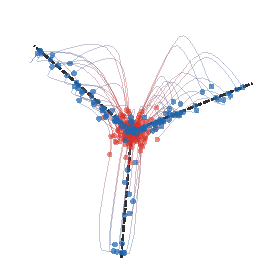
\includegraphics[width=.34\linewidth]{figures/gradflow-mlp-homogeneous-relu/neuron-trajectories.pdf} &
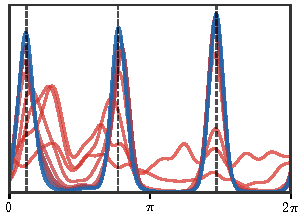
\includegraphics[width=.34\linewidth]{figures/gradflow-mlp-homogeneous-relu/direction-histogram.pdf}
\end{tabular}
\caption{Mean-field training of a homogeneous two-layer model as transport in neuron space. The left panel shows the Wasserstein particle gradient flow in the reduced homogeneous coordinates $(|u|v_1,|u|v_2)$, with black dashed rays marking the teacher directions. The right panel shows the weighted angular density along a front-loaded sequence of times, colored from red to blue, so that the early concentration of neuron directions is visible. The display follows the rendering of the auxiliary MLP experiment but keeps only the $W_2$ flow, not the spectral-flow comparison.}
\index{neuron}% strictindex
\index{two-layer neural network}% strictindex
\index{gradient!flow}% strictindex
\label{fig:gradflow-mlp-homogeneous-relu}
\end{figure}

\paragraph{Classical convexity and stationarity.}
\index{convexity!classical}% strictindex
\index{stationarity}% strictindex
Before using the specific homogeneity mechanism of Chizat and Bach, it is useful to isolate a simpler convex-analytic principle behind many mean-field arguments. Consider an energy of the form
\[
	F(\alpha)
	=
	\frac12\iint k(x,x')\d\alpha(x)\d\alpha(x')
	+
	\int V(x)\d\alpha(x)
	+C,
\]
on probability measures over a parameter domain. Assume that the quadratic part is convex in the classical sense, namely convex for the affine structure of measures:
\index{probability measure}% strictindex
\[
	Q((1-s)\alpha+s\beta)\leq (1-s)Q(\alpha)+sQ(\beta),
	\qquad
	Q(\alpha)=\frac12\iint k\d\alpha\d\alpha.
\]
This is ordinary convexity of the functional on the convex set of measures, not displacement convexity along $\Wass_2$ geodesics.
\index{convexity!along geodesics}% strictindex
\index{displacement!convexity}% strictindex

\begin{prop}[Affine convexity and stationary densities]\label{prop-classical-convex-stationary}
\index{convexity!classical}% strictindex
\index{stationary density}% strictindex
	Let $F=Q+\int V\,\d\alpha+C$ be as above, and assume that $Q$ is classically convex. Suppose that a Wasserstein gradient flow for $F$ converges to a measure $\alpha_\infty=\rho_\infty\d x$. Assume also the standard regularity needed to pass to the limit in the first variation, and assume that the support and positivity of $\rho_\infty$ allow the stationary condition to be tested against all admissible zero-mass density perturbations. In the form needed here, assume that this stationarity yields, for every competitor $\beta$, the variational inequality
\index{stationary condition}% strictindex
\index{first variation}% strictindex
\index{stationarity}% strictindex
\index{Wasserstein!gradient}% strictindex
\index{gradient!flow}% strictindex
\index{Wasserstein!gradient flow}% strictindex
	\[
		\int \delta F(\alpha_\infty)(x)\d(\beta-\alpha_\infty)(x)\geq0.
	\]
	Then $\alpha_\infty$ is a global minimizer of $F$.
\index{global!minimizer}% strictindex
\end{prop}
\begin{proof}[Proof sketch]
	The dissipation identity for the gradient flow gives stationarity of the limit: formally, after passing to the limit,
\index{gradient!flow}% strictindex
	\[
		\int \norm{\nabla \delta F(\alpha_\infty)}^2\d\alpha_\infty=0.
	\]
	Without such a support and positivity assumption, this identity only controls the first variation on the region explored by the limit. The density hypothesis allows one to test against sufficiently many signed density perturbations of total mass zero. By approximation and the assumed regularity, this yields the displayed first-order variational inequality for arbitrary competitors $\beta$. Classical convexity of $F$ in the affine variable $\alpha$ then gives the usual subgradient inequality
\index{subgradient inequality}% strictindex
\index{first variation}% strictindex
\index{convexity!classical}% strictindex
	\[
		F(\beta)\geq F(\alpha_\infty)
		+
		\int \delta F(\alpha_\infty)\d(\beta-\alpha_\infty)
		\geq F(\alpha_\infty).
	\]
	Thus no competitor has smaller energy. For square-loss two-layer mean-field models, \eqref{eq-mlp-square-loss-quadratic-linear} is exactly of this quadratic-plus-linear form, and positive semidefiniteness of the induced kernel $k$ is the classical convexity assumption.
\index{linear form}% strictindex
\index{two-layer neural network}% strictindex
\index{convexity!classical}% strictindex
\end{proof}

The mean-field description of two-layer training was developed in several works, including~\cite{ChizatBach2018OverparameterizedOT,MeiMontanariNguyen2018MeanFieldNN}. The distinctive contribution of Chizat and Bach is a global-convergence analysis for positively homogeneous networks without adding an explicit regularizer or relying on noisy SGD to create a Laplacian term. The following formal statement isolates the core mechanism and ignores the technical issues due to ReLU non-smoothness, support propagation and compactness.
\index{two-layer neural network}% strictindex

\begin{prop}[Formal global optimality for two-homogeneous mean-field flows]\label{prop-formal-chizat-bach}
\index{global!optimality}% strictindex
	Assume that the feature is positively two-homogeneous in the neuron variable,
\index{neuron}% strictindex
	\[
		\psi(\lambda x,z)=\lambda^2\psi(x,z)
		\qquad(\lambda>0),
	\]
	and that $f(\alpha)=J(G_\alpha)$ with $J$ convex and differentiable as a functional of the predictor. Let $\alpha$ be a smooth stationary point of the Wasserstein flow, so that $\nabla_x\delta f(\alpha)(x)=0$ on $\supp(\alpha)$. Assume also full directional support: for every nonzero direction $\omega$, the support of $\alpha$ intersects the ray $\{\lambda\omega:\lambda>0\}$. Then $\alpha$ is a global minimizer of $f$ over the mean-field model class.
\index{stationarity}% strictindex
\index{global!minimizer}% strictindex
\end{prop}
\begin{proof}
	Write
	\[
		h_\alpha(x)=\delta f(\alpha)(x)
		=
		\left\langle \nabla J(G_\alpha),\psi(x,\cdot)\right\rangle_\rho .
	\]
	By two-homogeneity of $\psi$, one has $h_\alpha(\lambda x)=\lambda^2h_\alpha(x)$. Normalize a nonzero direction $\omega$ and choose $r_\omega>0$ with $r_\omega\omega\in\supp(\alpha)$. Stationarity gives a zero radial derivative at this point:
	\[
		0=\frac{\d}{\d r}h_\alpha(r\omega)\bigg|_{r=r_\omega}
		=2r_\omega h_\alpha(\omega).
	\]
	Hence $h_\alpha(\omega)=0$ for every direction $\omega$, and by homogeneity $h_\alpha(x)=0$ for every $x$.

	For any competitor $\beta$, convexity of $J$ gives
	\[
		f(\beta)-f(\alpha)
		\geq
		\int h_\alpha(x)\d(\beta-\alpha)(x)=0.
	\]
	Thus no competitor has smaller risk. The rigorous theorem replaces the full directional support assumption by propagation and overparameterization hypotheses ensuring that a negative descent direction would be present in the support and would contradict stationarity.
\index{stationarity}% strictindex
\end{proof}
